\documentclass[border = .2cm]{standalone}
\usepackage{tikz}

\pgfdeclarelayer{bg}
\pgfsetlayers{bg,main}

\tikzstyle{vx}=[fill=gray!30, draw=black, shape=circle, minimum size=5pt, inner sep=2pt]
\tikzstyle{wire}=[-, thick]

\begin{document}
  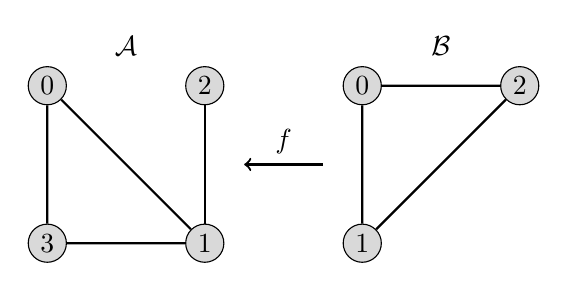
\begin{tikzpicture}
    \node [vx] (a0) at (-1, 1) {0};
    \node [vx] (a3) at (-1, -1) {3};
    \node [vx] (a2) at (1, 1) {2};
    \node [vx] (a1) at (1, -1) {1};
    \node at (0, 1.5) {$\mathcal{A}$};
    \node at (4, 1.5) {$\mathcal{B}$};

    \node [vx] (b0) at (3, 1) {0};
    \node [vx] (b1) at (3, -1) {1};
    \node [vx] (b2) at (5, 1) {2};

    \begin{pgfonlayer}{bg}
        \draw [wire] (a3) -- (a0) -- (a1) -- (a3);
        \draw [wire] (a1) -- (a2);
        \draw [wire] (b0) -- (b1) -- (b2) -- (b0);
        \draw [wire, ->] (2.5, 0) -- (1.5, 0) node[midway, above] {$f$};
    \end{pgfonlayer}
  \end{tikzpicture}
\end{document} 
